% BASIC SETTINGS 기본 세팅, 용지 사이즈, 등 필요할때 체크해서 수정해보자.
%조판이나 이런 단축키등 더 다양한 정보들은 내가 기록해둔 사이트를 참고해보자.
\documentclass[a4paper,12pt]{article} % Set paper size and document type
\usepackage{lmodern} % Use a slightly nicer looking font
\usepackage{url} % Proper formatting for URLs
\usepackage{graphicx} % Handle inclusion of non-PDF graphics
\usepackage{subfig} % Allow sub-figures inside a figure
\usepackage{enumitem} % Allow lists to pick up numbering where the last list left off
\usepackage{amsmath} %이 패키지는 amsmath로 수학적으로 나타낼때 매우 유리한 패키지이다.
\usepackage{kotex}%한국어를 지원 패키지.

% Change margins - default margins are too broad
\usepackage[margin=20mm]{geometry}

% SOURCE CODE LISTING SETTINGS 
% https://en.wikibooks.org/wiki/LaTeX/Source_Code_Listings
\usepackage{listings}
\usepackage{color}

% Color definitions for source code listings 
\definecolor{mygreen}{rgb}{0,0.6,0}
\definecolor{mygray}{rgb}{0.5,0.5,0.5}
\definecolor{mymauve}{rgb}{0.58,0,0.82}

% Formatting (line breaks, spacing, etc...) for code 파일 기본적인 포멧팅을 나타내는 옵션인 듯, 형식 그대로 쓸 거니, 필요한 것만 수정해서 쓰자.
\lstset{ 
  backgroundcolor=\color{white},   % choose the background color; you must add \usepackage{color} or \usepackage{xcolor}
  basicstyle=\footnotesize,        % the size of the fonts that are used for the code
  breakatwhitespace=false,         % sets if automatic breaks should only happen at whitespace
  breaklines=true,                 % sets automatic line breaking
  captionpos=b,                    % sets the caption-position to bottom
  commentstyle=\color{mygreen},    % comment style
  deletekeywords={...},            % if you want to delete keywords from the given language
  escapeinside={\%*}{*)},          % if you want to add LaTeX within your code
  extendedchars=true,              % lets you use non-ASCII characters; for 8-bits encodings only, does not work with UTF-8
  frame=single,	                   % adds a frame around the code
  keepspaces=true,                 % keeps spaces in text, useful for keeping indentation of code (possibly needs columns=flexible)
  keywordstyle=\color{blue},       % keyword style
  otherkeywords={*,...},           % if you want to add more keywords to the set
  numbers=left,                    % where to put the line-numbers; possible values are (none, left, right)
  numbersep=5pt,                   % how far the line-numbers are from the code
  numberstyle=\tiny\color{mygray}, % the style that is used for the line-numbers
  rulecolor=\color{black},         % if not set, the frame-color may be changed on line-breaks within not-black text (e.g. comments (green here))
  showspaces=false,                % show spaces everywhere adding particular underscores; it overrides 'showstringspaces'
  showstringspaces=false,          % underline spaces within strings only
  showtabs=false,                  % show tabs within strings adding particular underscores
  stepnumber=2,                    % the step between two line-numbers. If it's 1, each line will be numbered
  stringstyle=\color{mymauve},     % string literal style
  tabsize=2,	                   % sets default tabsize to 2 spaces
  title=\lstname                   % show the filename of files included with \lstinputlisting; also try caption instead of title
}


% Set document title and author 시작전 이름과, 날짜 등 남길 수 있는 방법.
\title{\LaTeX 사용법 \space{} Mathmatical method를 예로 나타내보자 \#1}
\author{MinWook Kang}
\date{2022-12-22} % If date is left blank, it will be hidden

% Document body ~문서의 시작을 알려주는 구문인 듯.
\begin{document}

\maketitle % Insert the title, author, and date

% 제목 적는 방법 (세션별로 나누는 것.)
\section{맥택스 사용방법} %  Create a section
일단, py 파일을 여기다가 옮기는 것을 해보자. 조판 단축키는 참고로 cmd + T이다.


%py 파일 삽입하는 방법
\vspace{5mm}
\lstinputlisting[language=Python]{example Bessel solution.py}
\vspace{5mm}


\noindent %이 구문은 글을 왼쪽으로 밀어 붙이는 기능.
여기다가 내용을 설명하고 위 코드에 대한 분석을 나타내면 될 듯.


% Include only specific lines from a file
\vspace{5mm}
\lstinputlisting[language=Python, firstline=19, lastline=20]{example Bessel solution.py}
\vspace{5mm}

\noindent 
이렇게 코드 전체에서 각 부분에 대한 설명을 계속해서 할 수 있음.

% Forces content onto the next page, useful for documents which should look nice when printed out
% 콘텐츠를 다음으로 넘기는 법
\clearpage

% Include code inline 인라인에 코드를 이렇게 남길 수 있다. 굳이 간단한 코드 자체를 표기하는 데에는 이런 방법도 있는 듯.
\vspace{5mm}
\begin{lstlisting}[language=Python]
print("Hi, I'm Python 3!")
\end{lstlisting}
\vspace{5mm}

%서브 세션 제목을 만드는 방법이다.
\subsection{Sub section for MacTex} % Create a subsection

\vspace{2mm} %제목과 거리를 둘 수 있는 방법 문단을 띄울때 쓰면 된다. 깔끔하게 이러한 것을 자주 이용하여 가독성을 높이자

%수식을 표현하는 방법을 나타내보자.
\vspace{2mm}

수식을 이렇게 나타낼 수 있다. 수식은 위키를 참고해서 익힐 수 있도록 하자.
% Format a mathematical expression
$$x' = x \cdot s cos \theta - y \cdot s sin \theta + t_x$$
$$y' = x \cdot s sin \theta + y \cdot s cos \theta + t_y$$
\vspace{2mm}


\noindent
이후에 나올 리스트를 이렇게 쓰면 가독성이 더 좋겠지.

% Make a list
\vspace{2mm}
\begin{enumerate}
\item I am the first thing in the list
\item I am the second thing in the list
\end{enumerate}
\vspace{2mm}

\noindent
여기에도 수식을 표현할 수 있음을 확인, 만약 $\sigma$에 대한 값을 보여줄려면,  "$4 \sigma_0$" using the "\$" sign. like this: 

\vspace{2mm}
$$u = (x - x_0) \frac{1}{4 \sigma_0} cos \theta_0 - (y - y_0) \frac{1}{4 \sigma_0} sin \theta_0 + 4 = (0 - 16) \frac{1}{4} - 0 + 4$$
\vspace{2mm}


\subsection{Sub section for MacTex}
%행렬도 이렇게 표현할 수 있다.

\vspace{2mm}
\[ \phi = \left\{ 
\begin{array}{l l}
\theta_0 + \theta_{pt} & if \ \theta_0 + \theta_{pt} \in [0,2 \pi)\\ 
\theta_0 + \theta_{pt} + 2 \pi & if \ \theta_0 + \theta_{pt} < 0\\
\theta_0 + \theta_{pt} - 2 \pi & if \ \theta_0 + \theta_{pt} \ge 2 \pi\\
\end{array} \right\}
\] 
\vspace{2mm}


\clearpage

\section{Second section}
%사진 넣는 법을 나타내 볼 것이다.

\vspace{5mm}
% Insert a figure with an image
\begin{figure}[!ht]
  \centering
  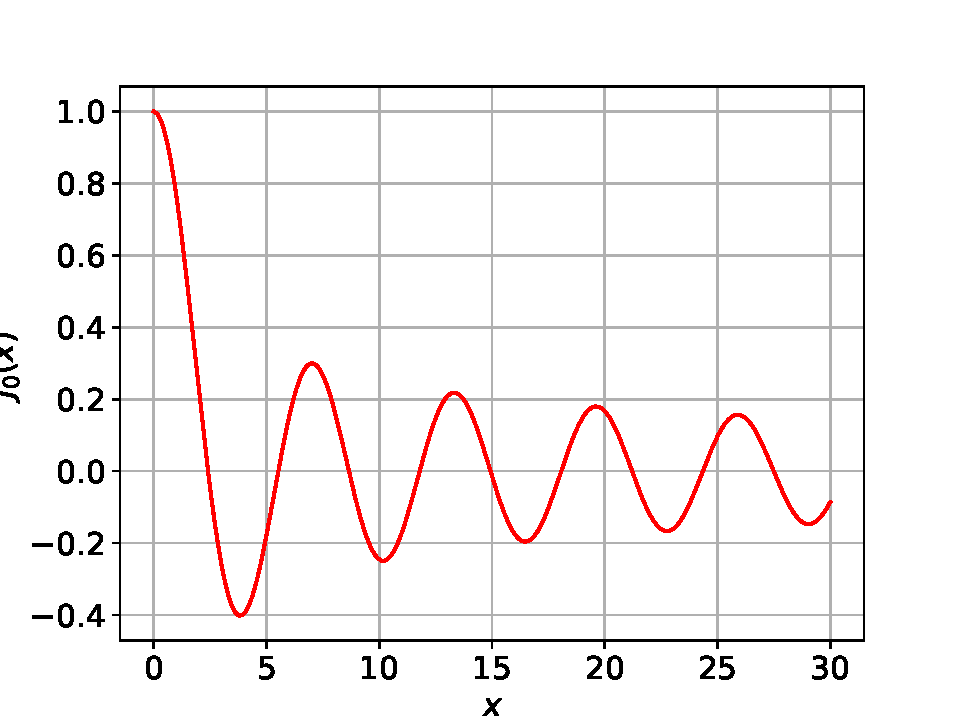
\includegraphics[width=0.5\textwidth]{12.pdf} %%세팅해서 안짤리게 확인
  \caption{Bessel Function}
\end{figure}

\noindent
%이번엔 행렬식을 표현해보자

\vspace{5mm}
\[ \left[ \begin{array}{c c c}
1.1754 & -0.8334 & 193.4191\\
0.2062 & 1.0380 & -141.0333\\
-0.0008 & 0.0007 & 1.0000\\
\end{array}
\right] \]
\vspace{5mm}

\noindent
%표도 나타낼 수 있다.

\vspace{5mm}
\noindent


\begin{tabular}{ |r|l| }
\hline
7C0 & hexadecimal \\
3700 & octal \\\cline{2-2}
11111000000 & binary \\
\hline \hline
1984 & decimal \\
\hline
\end{tabular}]

\vspace{5mm}

%각주를 나타내는 법도 적어본다.
\footnote{MinWook Kang}

\clearpage

\section{Thrid section}
\subsection{수식나타내기 연습을 해보자} % Create a subsection

Add $a$ squared and $b$ squaredto get $c$ squared. Or, usinga more mathematical approach

$$a^2 + b^2 = c^2$$
$$\lambda$$
$$\int $$

$$\forall x \in \mathbf{R}:
\qquad x^{2} \geq 0$$
\vspace{5mm}

$\lambda,\xi,\pi,\theta,\mu,\Phi,\Omega,\Delta$
\vspace{5mm}

$\sqrt{x} \Leftrightarrow x^{1/2}\quad \sqrt[3]{2}\quad \sqrt{x^{2} + \sqrt{y}}\quad \surd[x^2 + y^2]$
\vspace{5mm}

$\underbrace{\overbrace{a+b+c}^6
\cdot \overbrace{d+e+f}^7}
_\text{meaning of life} = 42$
\vspace{5mm}

\begin{equation*}
\sqrt{\frac{x^2}{k+1}}\qquad
x^\frac{2}{k+1}\qquad
\frac{\partial^2f}
{\partial x^2}
\end{equation*}

\vspace{5mm}
\begin{equation*}
\sum^n_{\substack{0<i<n \\
j\subseteq i}}
P(i,j) = Q(i,j)
\end{equation*}

\vspace{5mm}
\begin{multline}
a + b + c + d + e 
+f+ g + h + i
\\
= j + k + l + m + n
\end{multline}


\end{document}